\documentclass{standalone}
\usepackage{tikz}
\usetikzlibrary{arrows.meta, calc, decorations.pathmorphing, angles}

\begin{document}
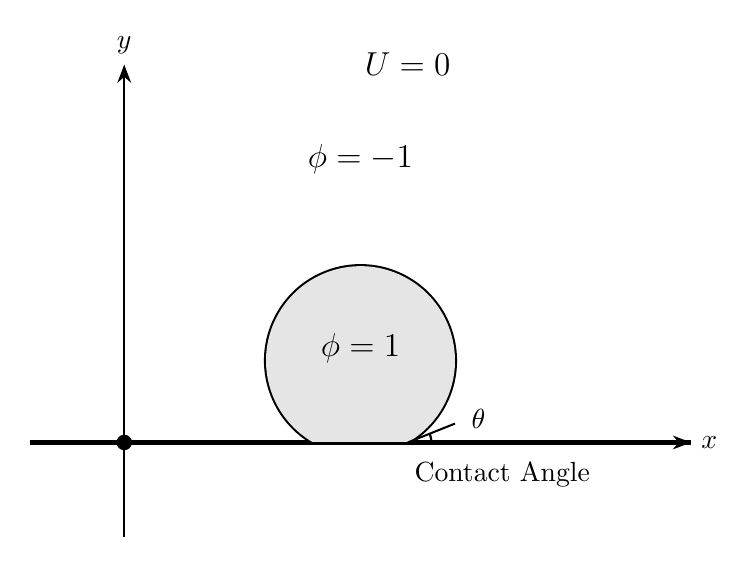
\begin{tikzpicture}[
    > = Stealth,
    thick,
    scale=1.2
]
    % Draw coordinate axes
    \draw[->, thick] (-1,0) -- (6,0) node[right] {$x$};
    \draw[->, thick] (0,-1) -- (0,4) node[above] {$y$};
    
    % Draw the plate (horizontal line)
    \draw[line width=1.5pt] (-1, 0) -- (6, 0);
    
    % Calculate points for the circle with 60-degree contact angle
    % For a 60-degree contact angle, we need a circle that meets the x-axis at 60 degrees
    \coordinate (left) at (2,0);
    \coordinate (right) at (3,0);
    
    % Draw a semi-circular droplet with contact angle of 60 degrees
    % We use a different center point to achieve the 60-degree angle
    \draw[line width=1.5pt] (left) arc (240:-60:1 and 1) -- cycle;
    
    % Fill droplet with light gray
    \begin{scope}
        \clip (left) arc (240:-60:1 and 1) -- cycle;
        \fill[black!10] (0,0) rectangle (6,10);
    \end{scope}
    
    % Add labels for phi values
    \node[font=\large] at (2.5,3) {$\phi = -1$};
    \node[font=\large] at (2.5,1) {$\phi = 1$};
    
    % Add U=0 label at the top
    \node[font=\large] at (3,4) {$U = 0$};
    
    % Label the contact lines
    % \node[below] at (1,-0.1) {Contact Line};
    \node[below] at (4,-0.1) {Contact Angle};
    
    % Draw and label the contact angle - mirrored on RIGHT side (below horizontal)
    % First draw a small horizontal line from the contact point
    \draw[line width=0.75pt] (right) -- ++(0.5,0);
    
    % Now draw the tangent line at 120 degrees (mirrored down from horizontal)
    \draw[line width=0.75pt] (right) -- ++(0.5,0.2); % tan(120°) = -tan(60°) ≈ -1.732, so y ≈ -0.433 for x = -0.25
    
    % Mark the angle with an arc
    \draw ($(right) + (0.25,0)$) arc (0:20:0.25);
    
    % Label the angle
    \node at (3.75,0.25) {$\theta$};
    
    % Add origin point
    \filldraw (0,0) circle (2pt);
\end{tikzpicture}
\end{document} 